\documentclass[../../sdf/tex/BPSK_system.tex]{subfiles}
\graphicspath{{../../images/}}
%opening
\onlyinsubfile{\title{Trans-Impedance Amplifier}}
\date{}

\begin{document}

\onlyinsubfile{\maketitle}

\subsection*{Introduction}

This super-block compresses the function of the following blocks:
\begin{itemize}
\item Ideal Amplifier;
\item White Noise
\item Add;
\item Pulse Shaper;
\end{itemize}
\noindent
This compression allows for a cleaner code. 

\subsection*{Input Parameters}

\begin{itemize}
	\item ElectricalNoiseSpectralDensity
	\item RollOffFactor
	\item ImpulseResponseTimeLength
	\item ImpulseResponseLength
	\item PassiveFilterMode
	\item SeeBeginningOfImpulseResponse
\end{itemize}

\subsection*{Functional Description}

The input signal is amplified, has white noise, with a user defined spectral density, added to it and is fed through a filter block. A diagram of the blocks that constitute this super-block, with the corresponding relations is presented in Figure~\ref{fig:physicalsystem}.

\begin{figure}[H]
\centering
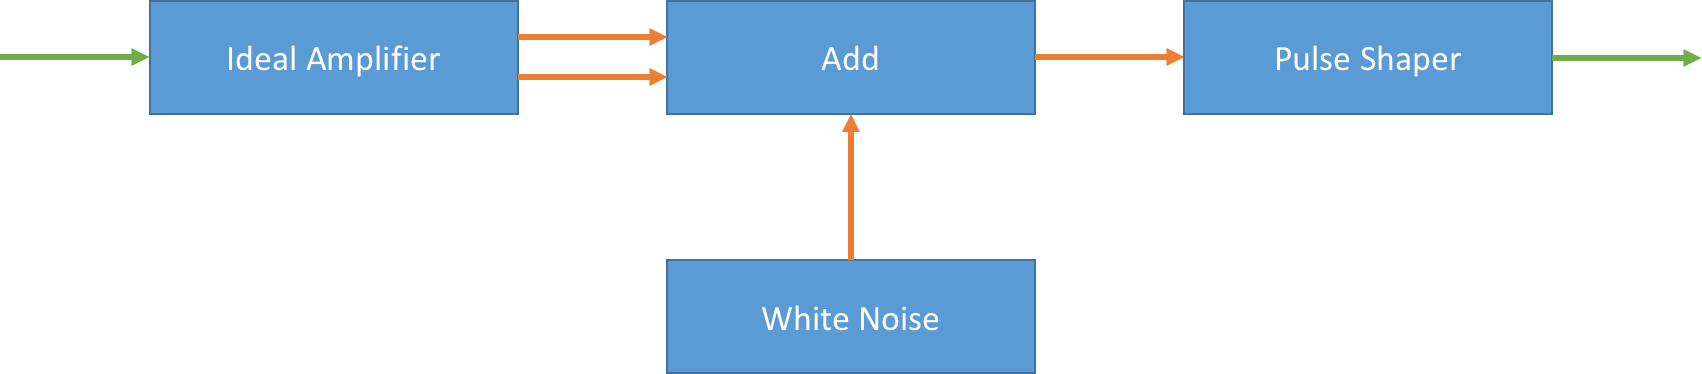
\includegraphics[width=\linewidth]{blockdiagram_amplifier.png}
\caption{Trans-Amplifier Block Diagram.}
\label{fig:physicalsystem}
\end{figure}

\subsection*{Inputs}

\textbf{Number}: 1

\textbf{Type}: Real, Complex or Complex\_XY signal (ContinuousTimeContinuousAmplitude)

\subsection*{Outputs}

\textbf{Number}: 1

\textbf{Type}: Real, Complex or Complex\_XY signal (ContinuousTimeContinuousAmplitude)

\end{document}